\subsection{Performance}
\subsubsection{Overview}
The main question in this section is whether the complete SSS SLAM data-processing pipeline can run in real time on the embedded test platform, not only whether the individual algorithms are efficient in isolation. This is important because a SLAM pipeline is only useful for onboard deployment if the full system can process incoming sensor data fast enough while sharing CPU time, memory, ROS2 communication, and periodic processing peaks with the other nodes.
\\ \\
This section evaluates the computational performance of the implemented SSS SLAM data-processing pipeline using the same standard parameters as in the previous result sections. The full ROS2 pipeline was executed together with the supporting middleware infrastructure, meaning that the measurements represent complete system behaviour rather than isolated algorithm benchmarks. This is important because the final performance depends on the interaction between nodes, message passing, memory usage, map size, update rates, and periodic processing steps.
\\ \\
The analysis is divided into runtime, CPU utilization, RAM usage, and schedulability. Runtime shows how the different parts of the pipeline behave during execution, while CPU and RAM show the resource demand on the embedded platform. Schedulability is the most important real-time benchmark, because it evaluates whether the measured execution times fit within the timing requirements of the pipeline. As will be shown, the system is strongly affected by parameter tuning, where changes such as map resolution cascade into later stages like feature extraction by reducing the number of map cells, memory load, required filter kernel sizes, and overall processing cost. This makes the pipeline highly tunable for different embedded platforms, while still showing that the implemented system can run in real time on constrained SBC hardware.



\newpage



\subsubsection{Runtime}
\begin{figure}[H]
    \centering
    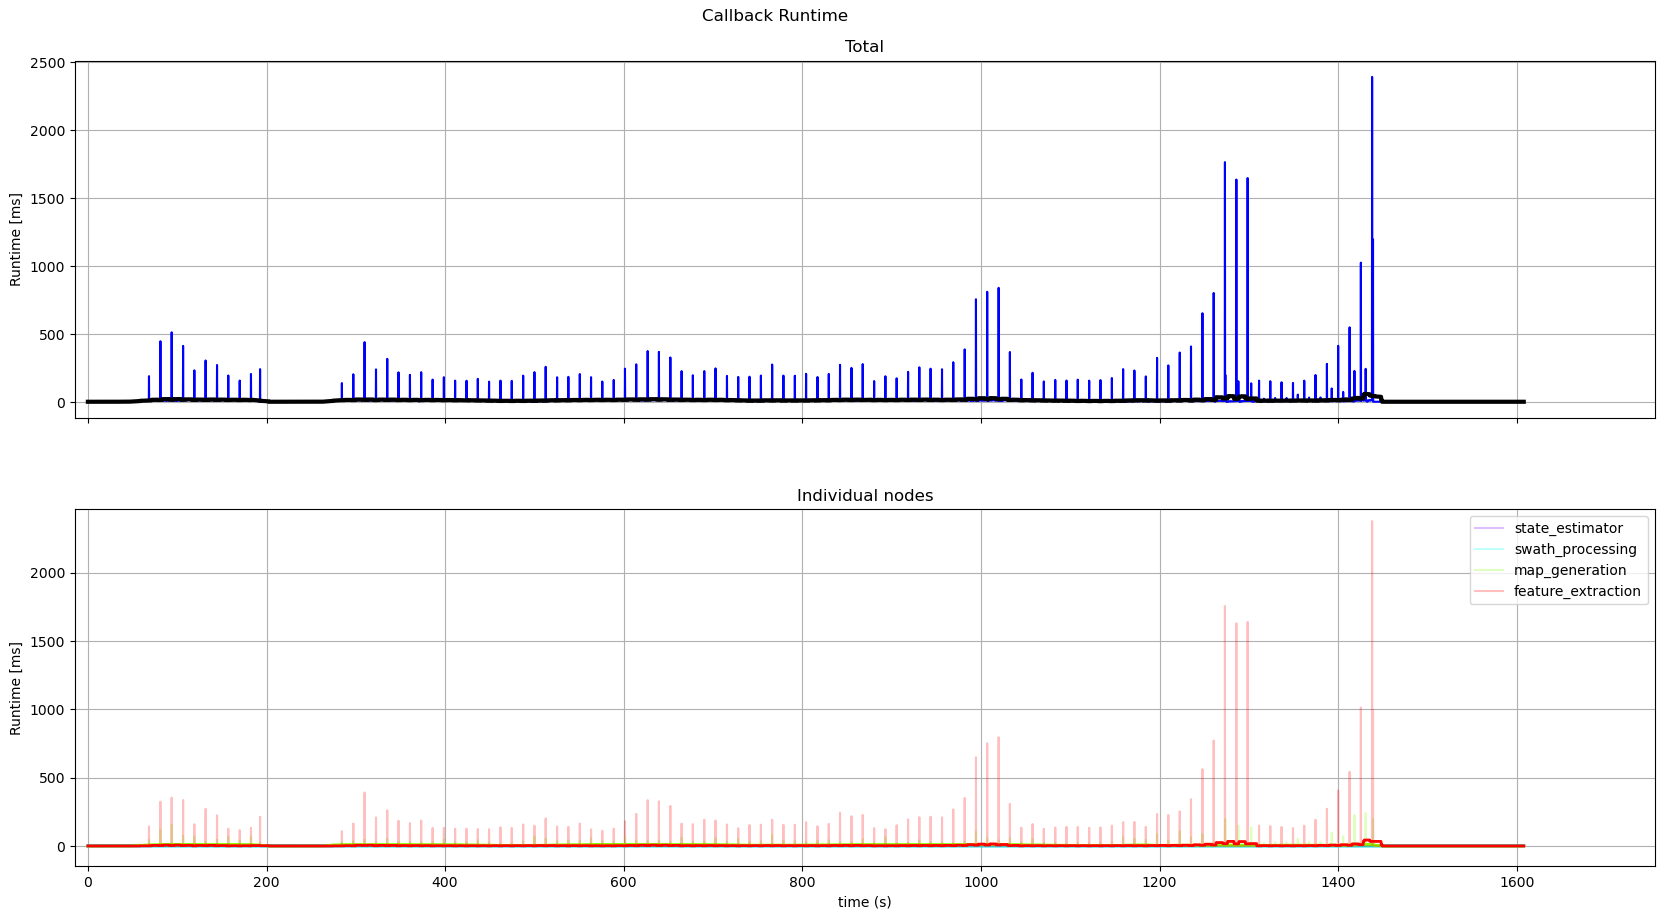
\includegraphics[width=1.0\linewidth]{Pictures/Results/Performance/Runtime.png}
    \caption{Runtime of the full SSS SLAM data-processing pipeline and the individual node execution times.}
    \label{fig:results-performance-runtime}
\end{figure}
\noindent
The runtime behaviour of the complete SSS SLAM data-processing pipeline is shown in Figure \ref{fig:results-performance-runtime}. Most of the runtime remains low during normal operation, where swaths are continuously processed and inserted into the local probabilistic map. The largest runtime peaks occur when a complete local map is extracted and passed to the feature extraction stage. This is expected, since feature extraction operates on the full generated map image and must process a much larger memory region than the individual swath update steps.
\\ \\
It is important to note that these runtime peaks do not directly mean that feature extraction is the dominant real-time bottleneck. Feature extraction and map extraction are computationally heavier per execution, but they only run periodically when a local map is ready. In contrast, swath processing and map generation have smaller runtime values, but are executed much more frequently as new sonar data arrives. Therefore, this plot mainly shows the execution behaviour of the pipeline and where the periodic peaks occur. The actual real-time feasibility is evaluated more directly in the schedulability analysis later in this section.



\newpage



\subsubsection{CPU}
\begin{figure}[H]
    \centering
    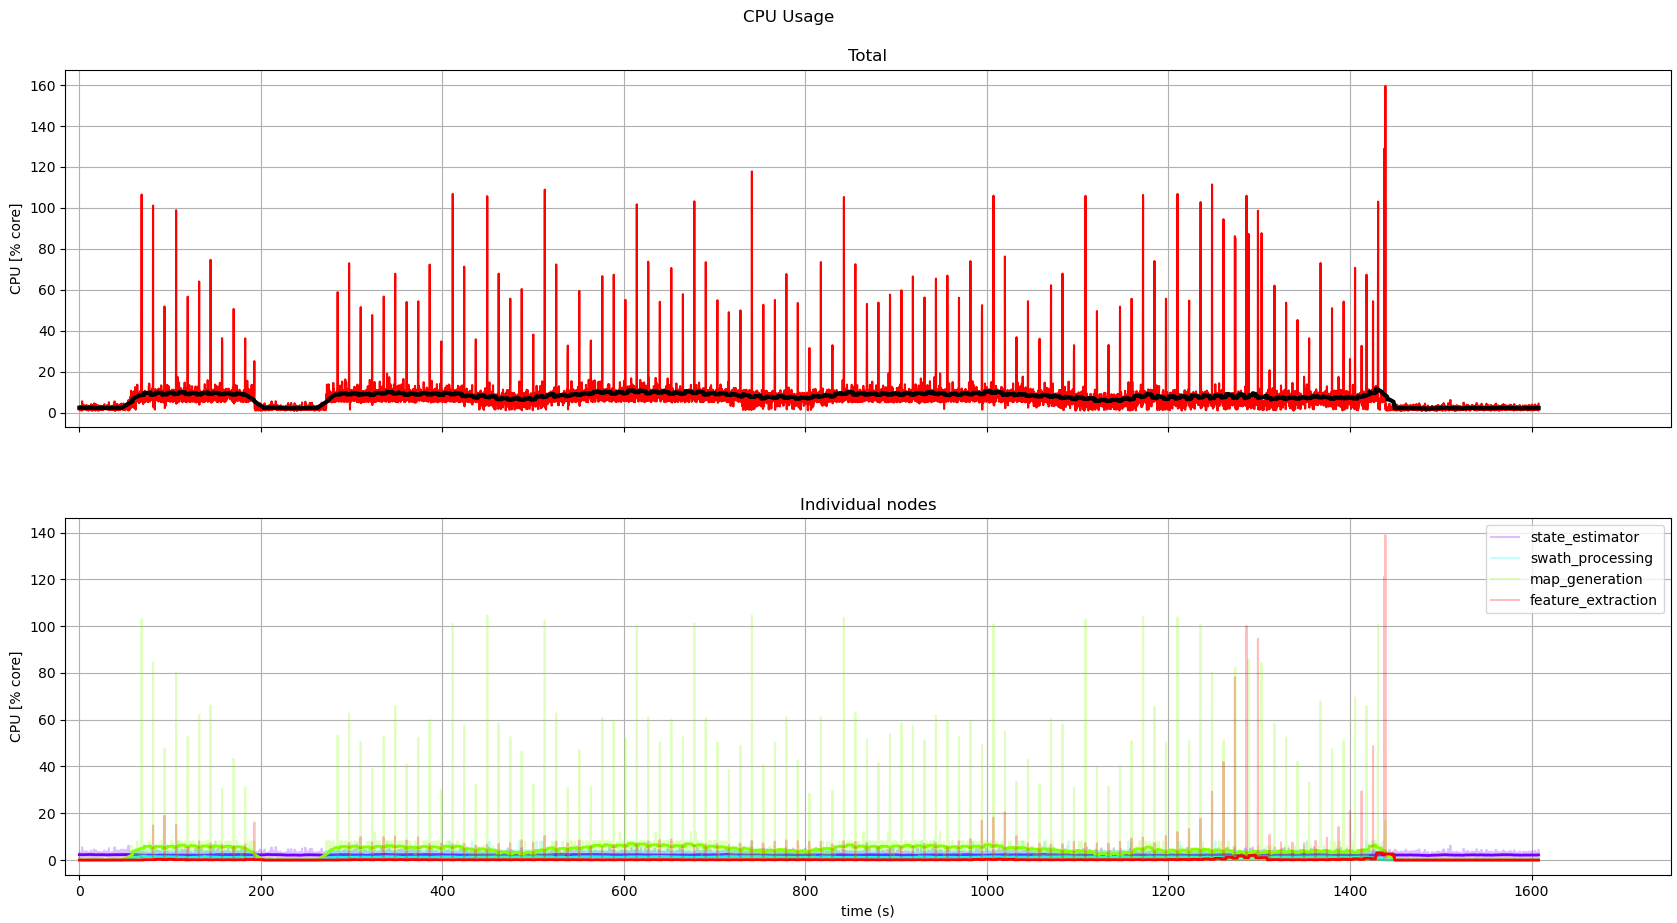
\includegraphics[width=1.0\linewidth]{Pictures/Results/Performance/CPU.png}
    \caption{CPU load of the full SSS SLAM data-processing pipeline and the individual node loads.}
    \label{fig:results-performance-cpu}
\end{figure}
\noindent
The CPU utilization of the complete SSS SLAM data-processing pipeline is shown in Figure \ref{fig:results-performance-cpu}. The results show the total CPU load of the full pipeline together with the contribution from the individual nodes. From the observed CPU load, the system appears to remain well within the available compute budget of the Raspberry Pi 4 Model B. The load indicates that the complete data-processing pipeline should comfortably fit within 2 CPU cores, leaving additional compute resources available for the remaining SLAM back-end, logging, visualization, or other onboard software.
\\ \\
However, CPU utilization alone is not sufficient to make a final real-time conclusion. A system can have low average CPU load while still missing timing requirements if some tasks execute too late or if periodic peaks overlap badly. Therefore, the CPU results should be interpreted as an indication of available computational headroom, while the final real-time feasibility is evaluated more directly in the schedulability analysis later in this section.



\newpage



\subsubsection{RAM}
\begin{figure}[H]
    \centering
    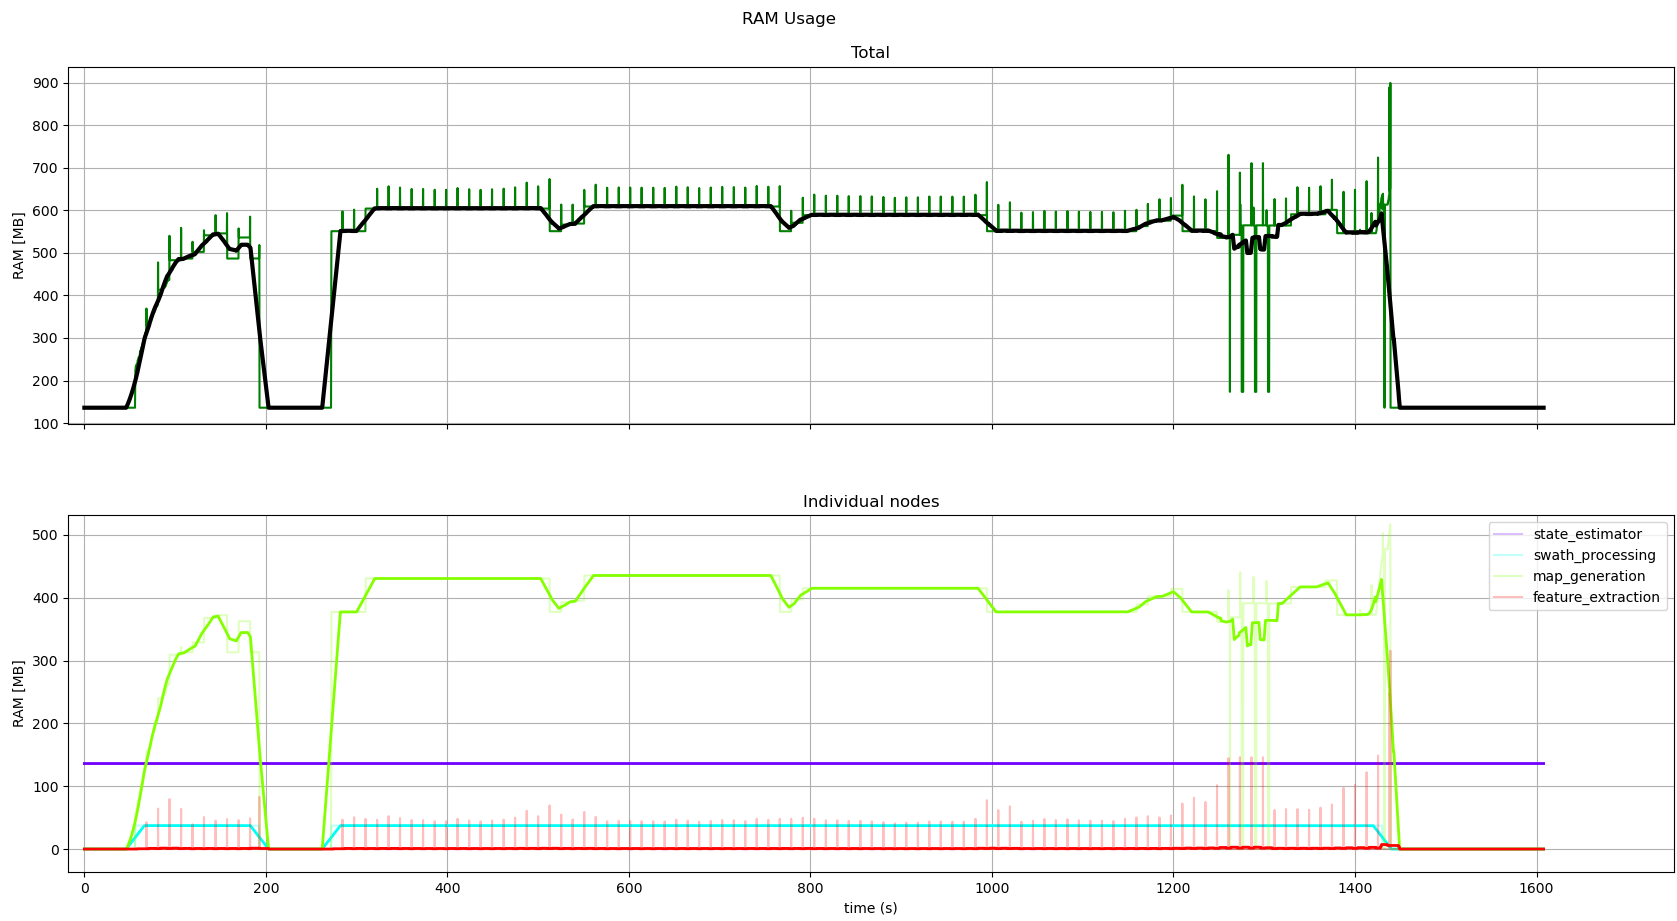
\includegraphics[width=1.0\linewidth]{Pictures/Results/Performance/RAM.png}
    \caption{RAM usage of the full SSS SLAM data-processing pipeline and the individual node memory.}
    \label{fig:results-performance-ram}
\end{figure}
\noindent
The RAM usage of the complete SSS SLAM data-processing pipeline is shown in Figure \ref{fig:results-performance-ram}. The full pipeline peaks at close to $1\,\mathrm{GB}$ of RAM, which is expected since the system must keep the active local map, map chunks, buffered swaths, and intermediate image data in memory while new map regions are generated and updated. The memory demand is therefore mainly caused by the local map generation and feature extraction stages, where large map images and temporary processing buffers are required.
\\ \\
The RAM usage remains mostly stable throughout the run, with only smaller periodic increases when a complete local map is passed to the feature extraction stage. These spikes occur because feature extraction needs to load and process the full map image using filtering, segmentation, and landmark detection operations. The stable baseline indicates that the chunk based map management and bounded local map representation successfully prevent unbounded memory growth during operation. Since the Raspberry Pi used in the experiment has $4\,\mathrm{GB}$ of RAM, the measured memory usage leaves a comfortable margin and shows that the pipeline is suitable for embedded SBC hardware with limited memory resources.



\newpage



\subsubsection{Schedulability Analysis}
\begin{figure}[H]
    \centering
    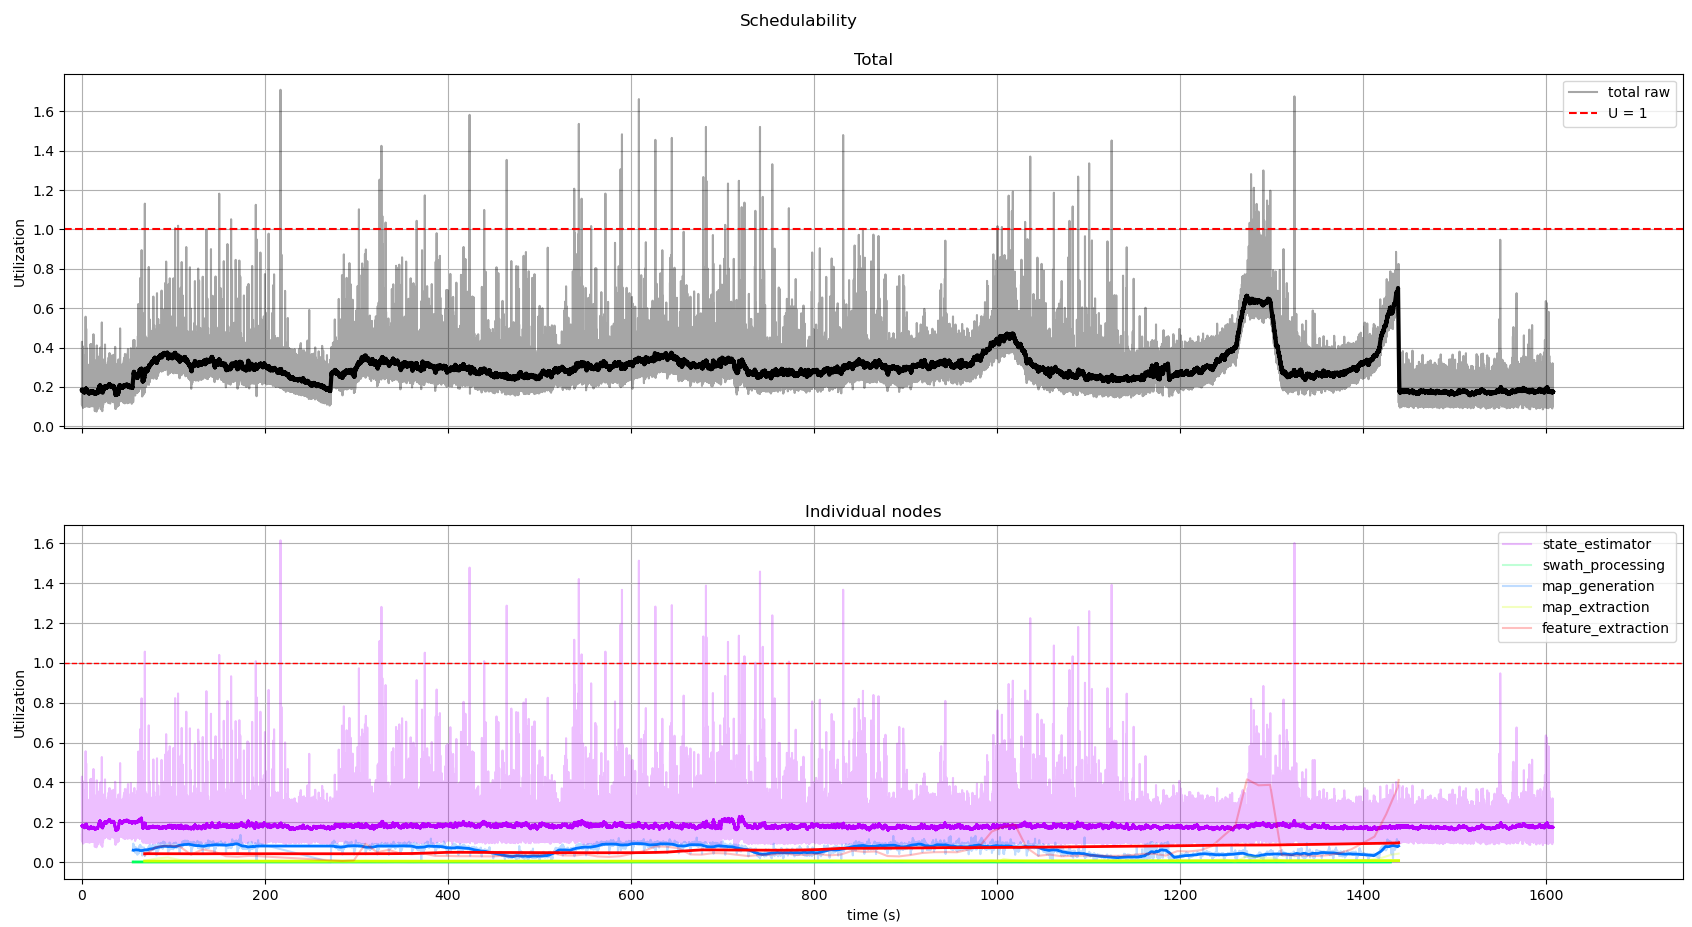
\includegraphics[width=1.0\linewidth]{Pictures/Results/Performance/Schedulability.png}
    \caption{Schedulability analysis of the full SSS SLAM data-processing pipeline including the state estimator.}
    \label{fig:results-performance-schedulability}
\end{figure}
\noindent
The schedulability analysis with the full SSS SLAM data-processing pipeline is shown in Figure \ref{fig:results-performance-schedulability}. Since the experiments were performed on a standard Ubuntu installation using the default Linux EEVDF scheduler, formal hard real-time schedulability cannot be guaranteed. However, the measured runtime traces can still be used for practical deadline risk and utilization analysis. Here, utilization is estimated from the measured execution time of each processing step relative to the time until that same step must run again. This gives a more realistic indication of real-time load than runtime alone.
\\ \\
For this analysis, the map generation node is separated into map generation and map extraction. Map generation refers to the frequent insertion of incoming sonar swaths into the probabilistic map, while map extraction refers to the less frequent operation where the complete local map is reconstructed and passed to feature extraction. This separation is important because map generation runs often with low runtime, while map extraction creates larger periodic peaks. Keeping them separate gives a clearer representation of the actual real-time behaviour of the pipeline.
\\ \\
The total utilization in Figure \ref{fig:results-performance-schedulability} is observed to hover slightly above $1.0$, indicating that the complete data-processing pipeline requires more than 1 CPU core and should therefore be scheduled across at least 2 cores. An important observation is that the state estimator contributes strongly to the utilization, even though its individual runtime is small. This is caused by the high IMU update rate, where small execution times accumulate significantly because the estimator runs many times per second. In contrast, sonar based processing runs at a much lower rate. Feature extraction and map extraction have larger individual runtimes, but occur only periodically, so their schedulability contribution is lower than the runtime plot alone might suggest.
\begin{figure}[H]
    \centering
    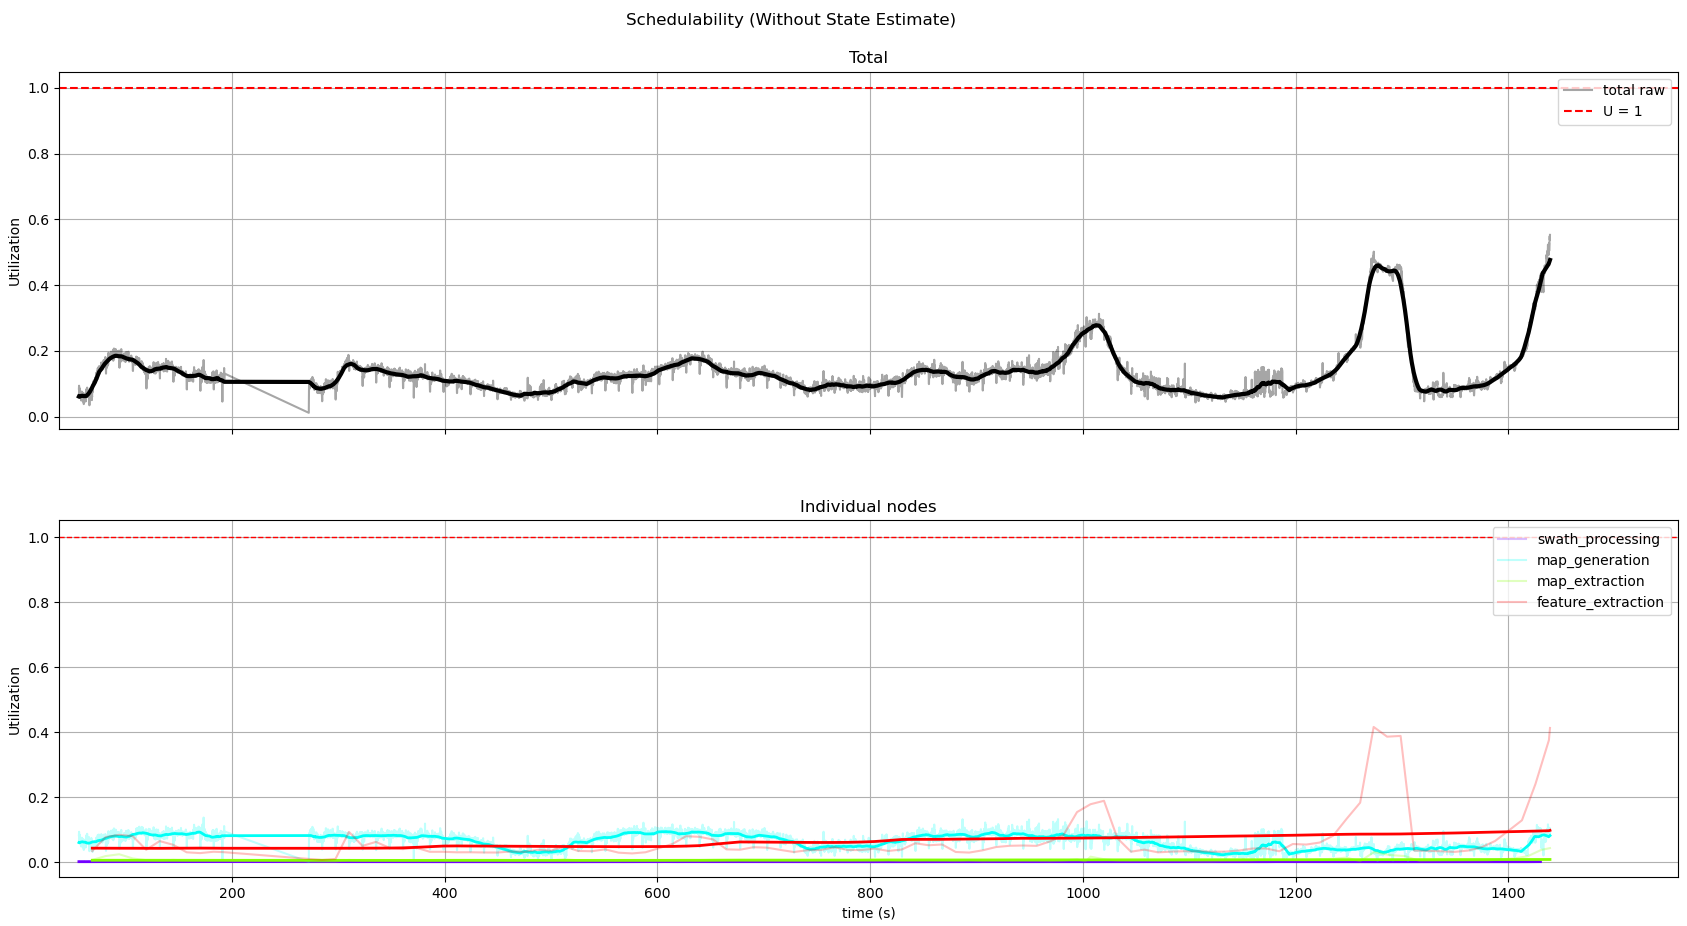
\includegraphics[width=1.0\linewidth]{Pictures/Results/Performance/Schedulability_NO_state_estimate.png}
    \caption{Schedulability analysis of the local map generation pipeline without the state estimator contribution.}
    \label{fig:results-performance-schedulability-no-state-estimate}
\end{figure}
\noindent
When the state estimator is considered separately, as shown in Figure \ref{fig:results-performance-schedulability-no-state-estimate}, the remaining local map generation pipeline stays below $1.0$ utilization. This suggests that, in practice, 1 of Raspberry Pis cores could be dedicated to the state estimator, while another core can handle swath processing, map generation, map extraction, and feature extraction, all on the same Raspberry Pi, but separate cores. The remaining 2 cores on the Raspberry Pi 4 are then available for the SLAM front-end and back-end, preintegration, logging, visualization, or other onboard processes. This is an important result, as it indicates that the implemented SSS SLAM data-processing pipeline is real-time capable on constrained embedded SBC hardware.



\newpage



\subsubsection{Tuned Pipeline Performance}
The previous results show that the full SSS SLAM data-processing pipeline can run in real time on the Raspberry Pi 4, with 1 core effectively sufficient for the state estimator and 1 core sufficient for the local map generation pipeline. However, many embedded systems may have stricter compute or memory limits than this test platform. Therefore, an additional tuned experiment was performed to evaluate how the pipeline behaves when the computational load is deliberately reduced. The same dataset and default configuration were used, except for the parameters listed in Table \ref{tab:results-performance-tuned-parameters}. The main change is that the map resolution is reduced from $0.03\,\mathrm{m/pixel}$ to $0.06\,\mathrm{m/pixel}$, and landmark height estimation is disabled.
\begin{table}[H]
    \centering
    \caption{Changed parameters used for the tuned pipeline experiment. All other parameters are unchanged from the standard configuration.}
    \label{tab:results-performance-tuned-parameters}
    \begin{tabular}{l l}
        \hline
        Parameter & Value \\
        \hline

        \multicolumn{2}{l}{\textbf{State estimation}} \\
        All parameters & Unchanged \\
        \\[-0.6em]

        \multicolumn{2}{l}{\textbf{Swath processing}} \\
        All parameters & Unchanged \\
        \\[-0.6em]

        \multicolumn{2}{l}{\textbf{Map generation}} \\
        Map resolution & 0.06 m/pixel \\
        \\[-0.6em]

        \multicolumn{2}{l}{\textbf{Feature extraction}} \\
        Bilateral filter diameter & 15 pixels \\
        Semantic local window size & 31 pixels \\
        Semantic support search radius & 13 pixels \\
        Minimum semantic support & 70 pixels \\
        Minimum landmark area & 2000 pixels \\
        Height estimation enabled & false \\

        \hline
    \end{tabular}
\end{table}
\noindent
Most of the tuned feature extraction parameters are reduced compared to the standard configuration. This is expected, since lowering the map resolution means that the same physical area is represented by fewer pixels. As a result, filters, local windows, search radius, and minimum support thresholds can also be reduced while still covering approximately the same physical structures. The effect is not purely linear and still requires empirical tuning, but the important point is that reducing the map resolution also reduces the cost of later processing stages. This gives a cascading performance improvement, smaller maps require less memory, smaller image processing kernels, fewer pixel operations, and lower feature extraction runtime. The tradeoff is reduced spatial detail, so map resolution should not be lowered too far. If the resolution becomes too coarse, small landmarks and fine geometric structures will be lost, making both map generation and feature extraction less reliable.

\newpage

\begin{figure}[H]
    \centering
    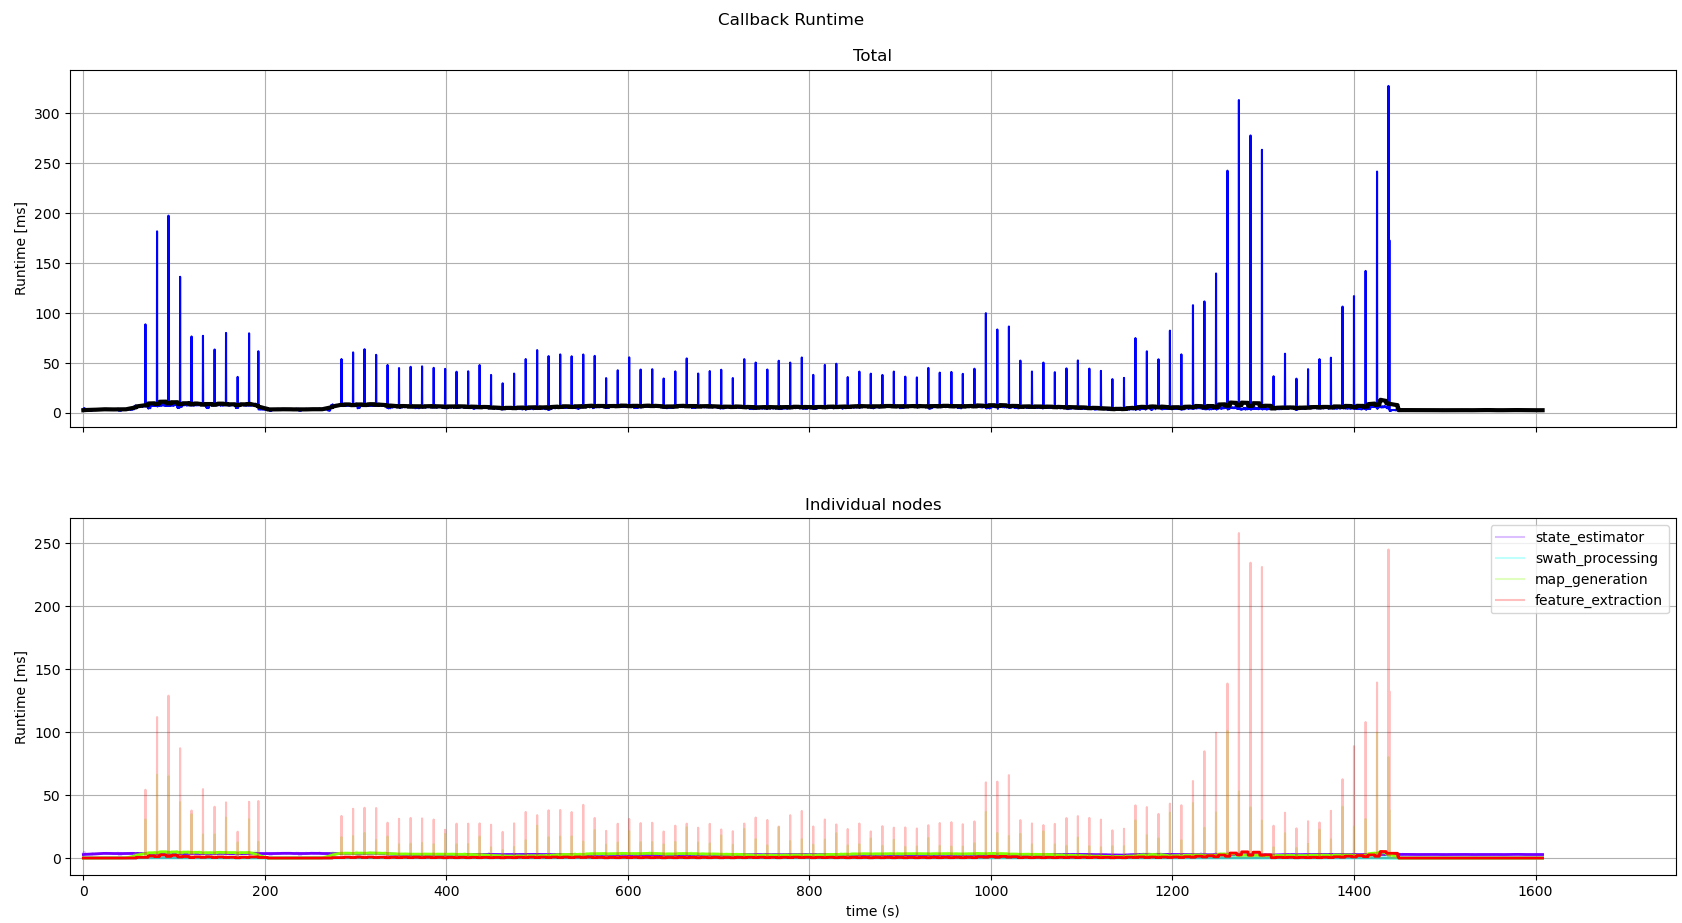
\includegraphics[width=1.0\linewidth]{Pictures/Results/Performance/Runtime_TUNED.png}
    \caption{Runtime of the tuned SSS SLAM data-processing pipeline and the individual node execution times.}
    \label{fig:results-performance-runtime-tuned}
\end{figure}

\begin{figure}[H]
    \centering
    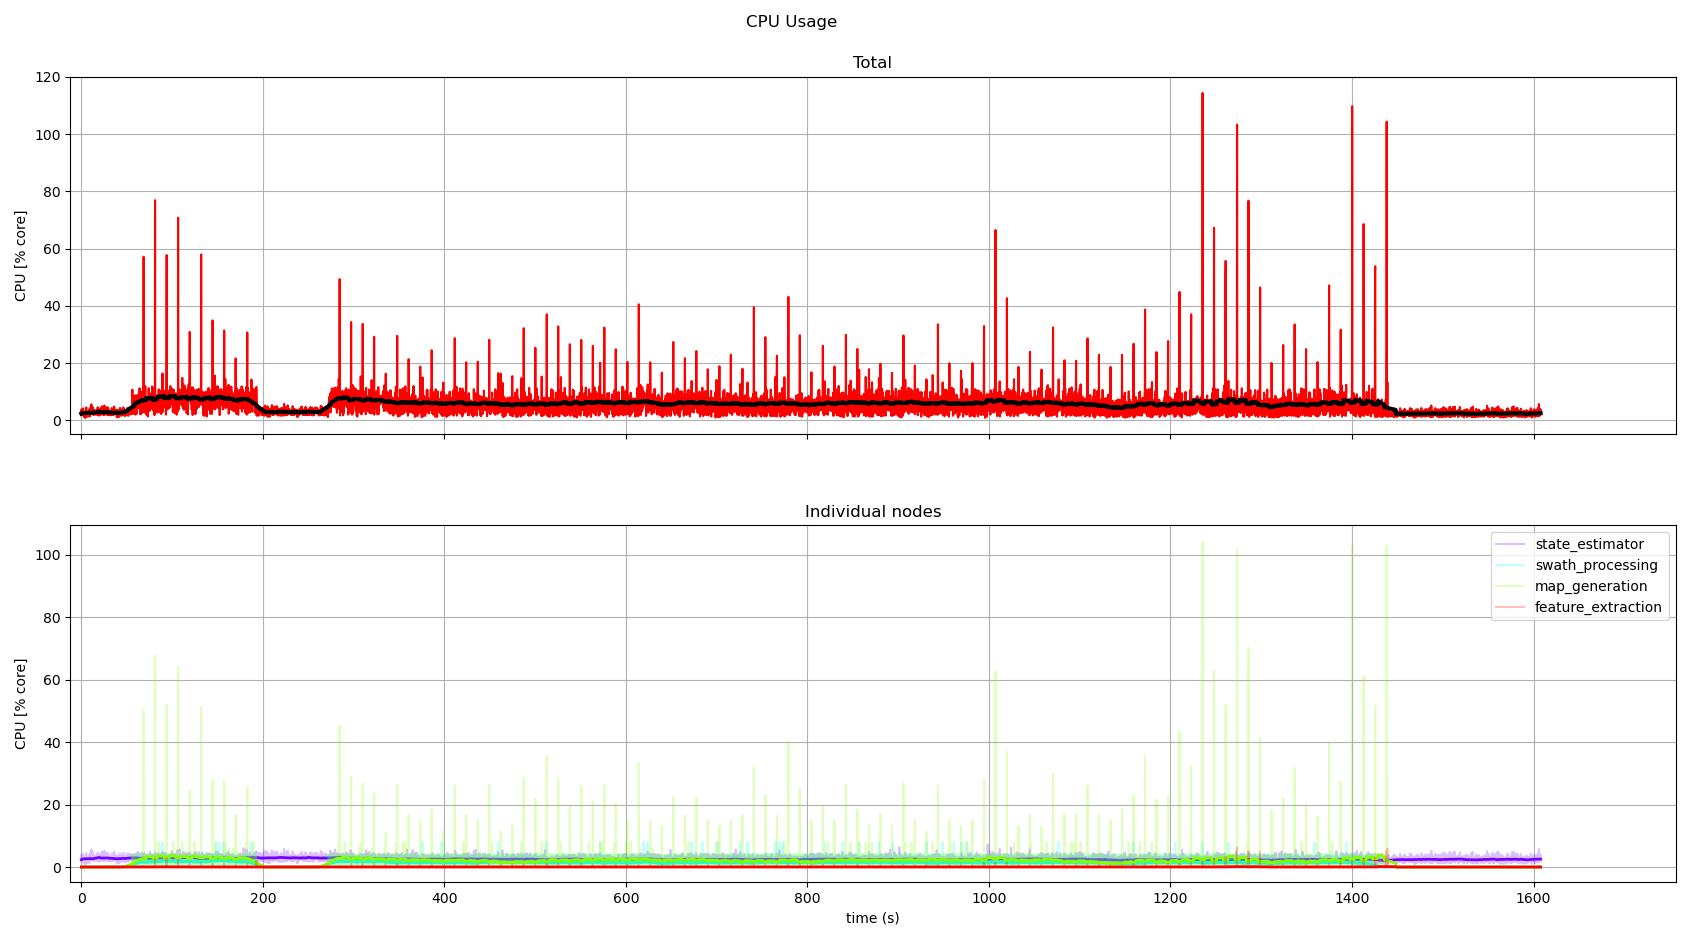
\includegraphics[width=1.0\linewidth]{Pictures/Results/Performance/CPU_TUNED.png}
    \caption{CPU load of the tuned SSS SLAM data-processing pipeline and the individual node loads.}
    \label{fig:results-performance-cpu-tuned}
\end{figure}

\newpage

\begin{figure}[H]
    \centering
    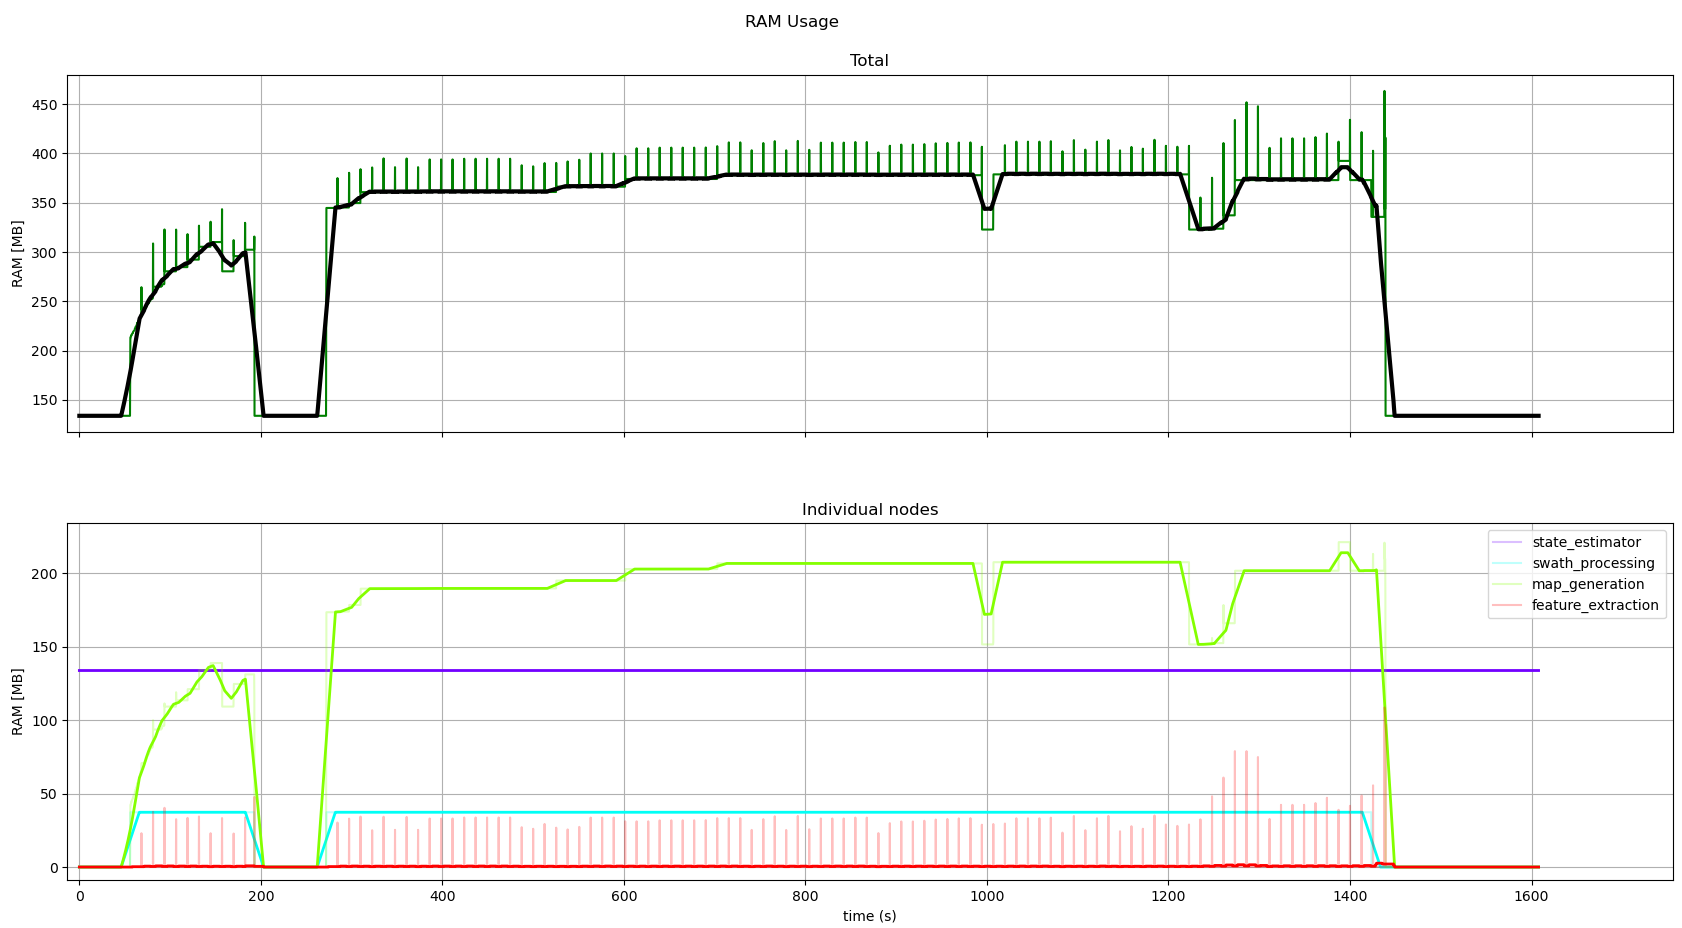
\includegraphics[width=1.0\linewidth]{Pictures/Results/Performance/RAM_TUNED.png}
    \caption{RAM usage of the tuned SSS SLAM data-processing pipeline and the individual node memory.}
    \label{fig:results-performance-ram-tuned}
\end{figure}

\begin{figure}[H]
    \centering
    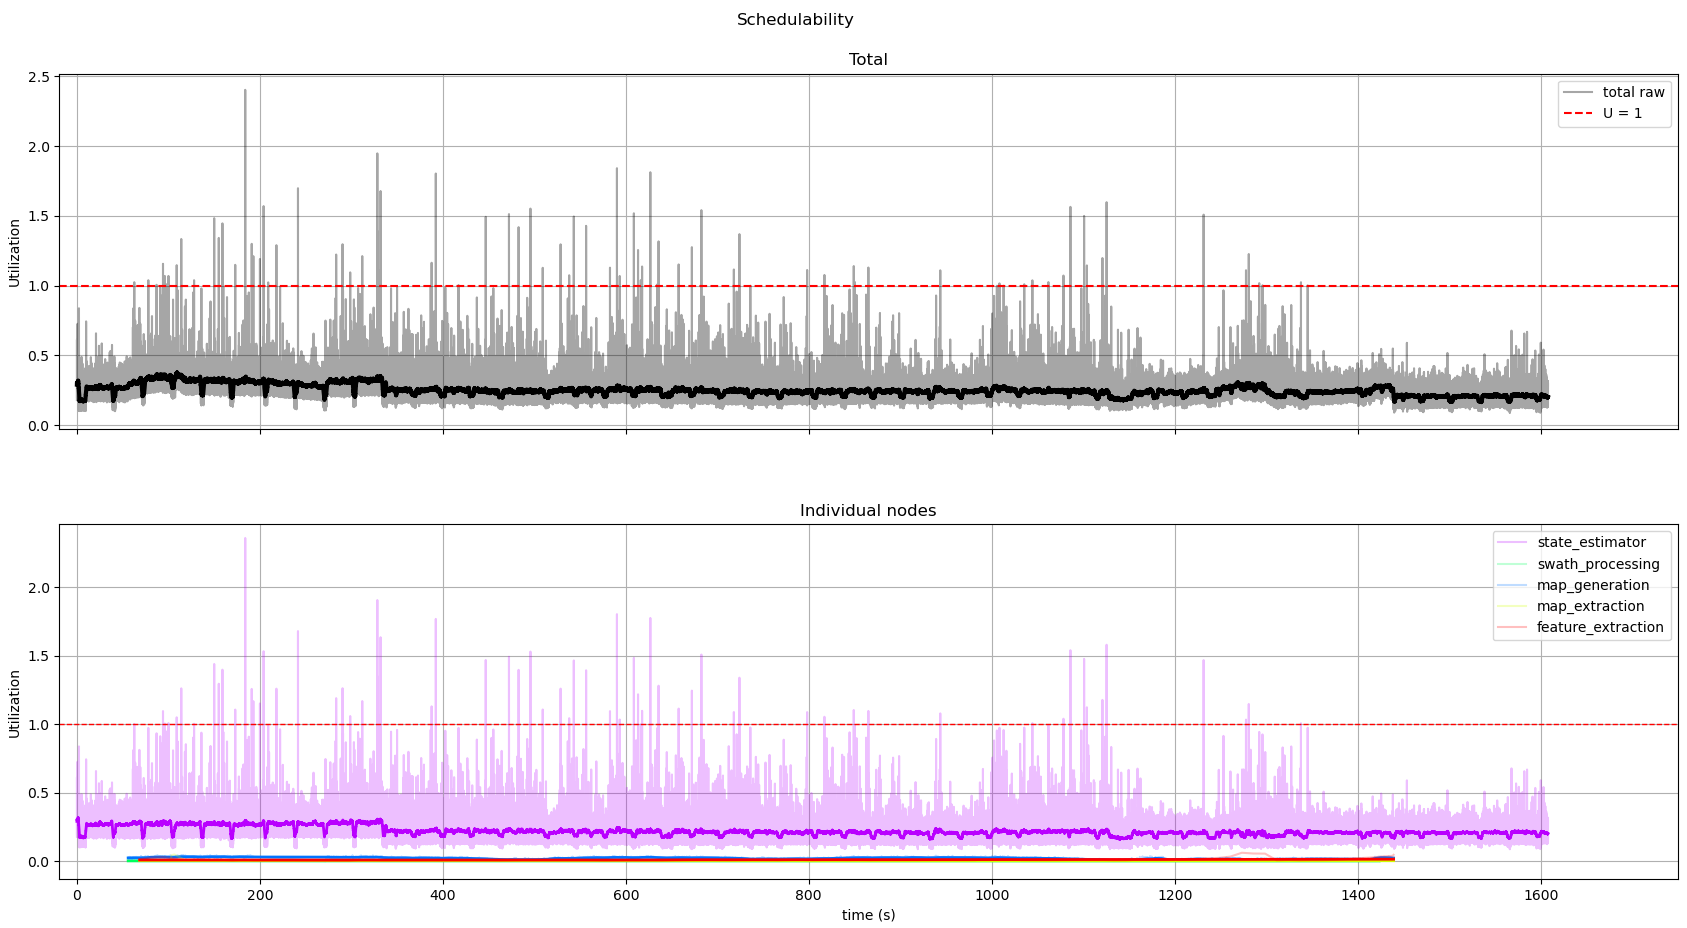
\includegraphics[width=1.0\linewidth]{Pictures/Results/Performance/Schedulability_TUNED.png}
    \caption{Schedulability analysis of the tuned SSS SLAM data-processing pipeline including the state estimator.}
    \label{fig:results-performance-schedulability-tuned}
\end{figure}

\newpage

\begin{figure}[H]
    \centering
    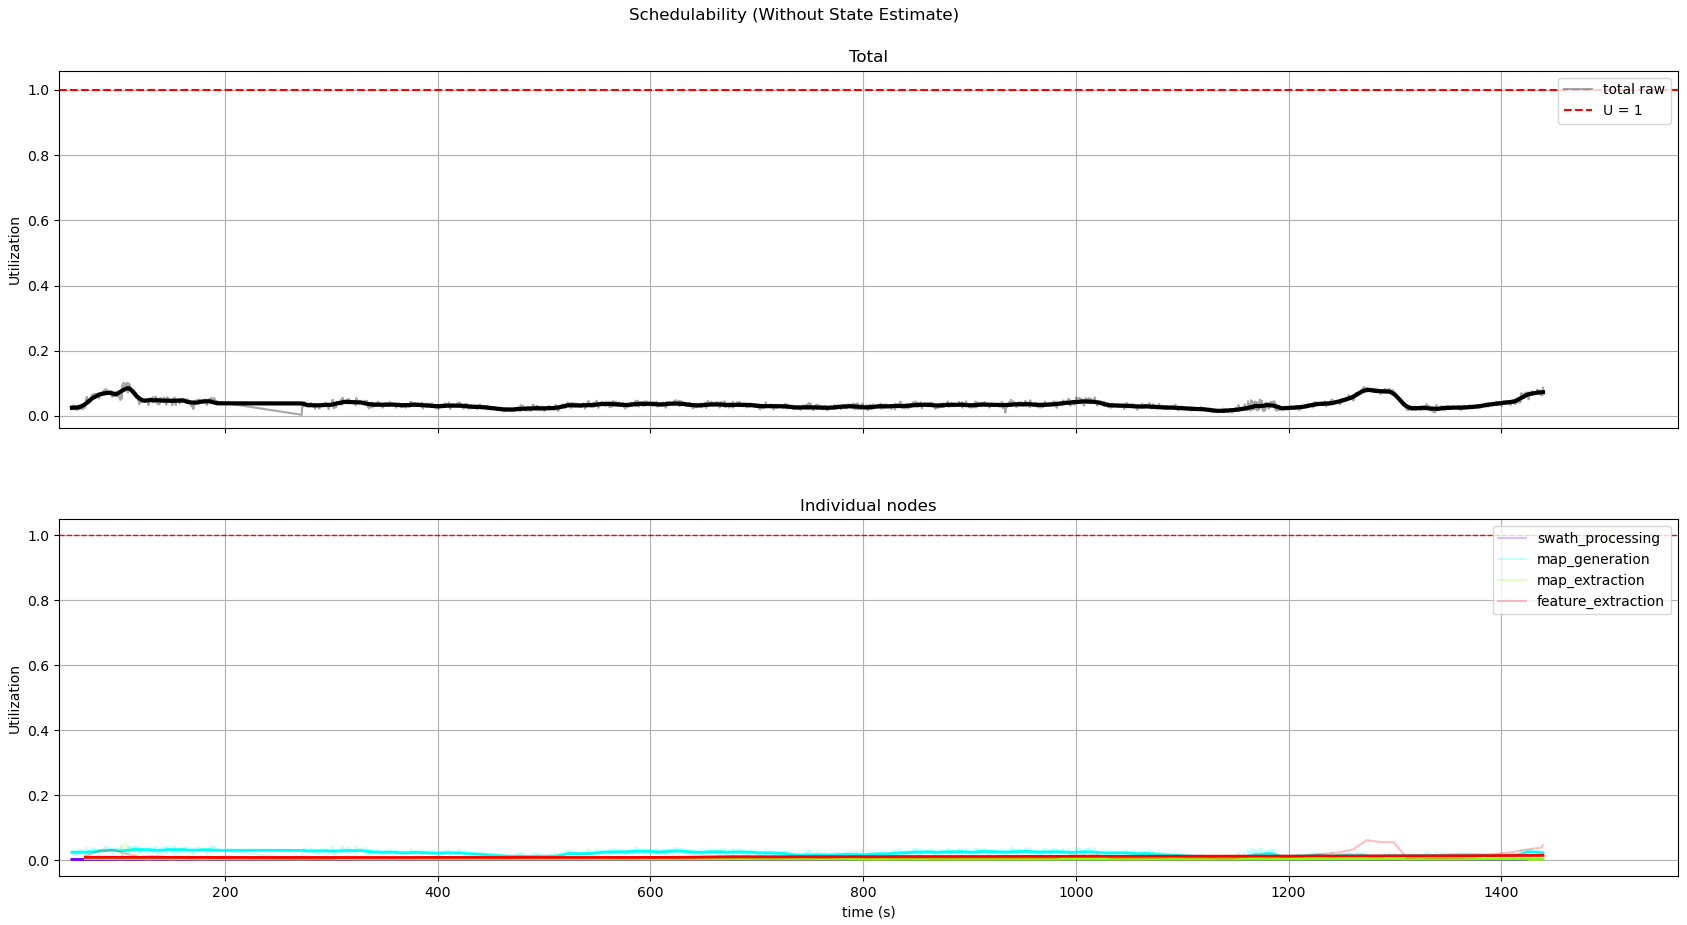
\includegraphics[width=1.0\linewidth]{Pictures/Results/Performance/Schedulability_NO_state_estimate_TUNED.png}
    \caption{Schedulability analysis of the tuned local map generation pipeline without the state estimator contribution.}
    \label{fig:results-performance-schedulability-no-state-estimate-tuned}
\end{figure}
\noindent
The tuned results show a large reduction in resource usage. As expected, halving the map resolution approximately halves the memory usage, reducing the full pipeline RAM demand from close to $1\,\mathrm{GB}$ to around $0.5\,\mathrm{GB}$. The schedulability improvement is even stronger, since the utilization peaks are reduced from roughly $50\%$ to around $10\%$ for the local map generation pipeline. This shows that the performance gain is larger than the memory reduction alone, because the smaller map also reduces the cost of feature extraction and other image processing steps. The exact real-time behaviour will always depend on the platform and scheduler, but these results show that the pipeline is highly tunable and can be adapted to stricter embedded compute budgets. With the tuned configuration, the local map generation pipeline becomes light enough that even more constrained SBC hardware could run it comfortably, and with a more efficient state estimator the complete SLAM data-processing pipeline could potentially fit on a single CPU core.
\\ \\
This is an important finding, as it shows that the implemented pipeline is not only real-time capable on the tested platform, but can also be scaled and tuned for more constrained embedded systems.
